\chapter{Knot selection in spline models: cannabis dependence}
\label{applications-splines_knot_loc}

The meta-analysis of data from systematic review of the prevalence of
cannabis dependence has a clear age-pattern, providing an example of
the importance of knot selection in spline models.

Symptoms associated with cannabis dependence are compulsive use and
difficulty with abstinence.  The American Psychiatric Association
recognizes cannabis dependence as fulfilling three or more of the
following seven substance dependence criteria: \cite{american_diagnostic_2000, coffey_cannabis_2002}
    \begin{itemize} \label{page:app-substance_dependence}
        \item tolerance;
        \item withdrawal;
        \item substance is taken in larger amounts or over longer
          period than intended;
        \item persistent desire or unsuccessful efforts to control
          substance use;
        \item great deal of time is spent to obtain, use, or recover
          from effects of substance;
        \item important social, occupational, or recreational
          activities are reduced because of substance use;
        \item continued substance use despite knowledge of
          physiological or psychological problems induced by substance
          use.
    \end{itemize}

Despite a large body of data on cannabis \emph{use}, there is little
data available on the descriptive epidemiology of cannabis
dependence.\cite{Degenhardt_GBDrugs_2011} Systematic review yielded
fifty-three rows of prevalence data were identified for cannabis
dependence prevalence, covering 3 regions.  For this example, we have
restricted our attention to only data from USA (Figure
\ref{fig:app-cannabis_data}).

    \begin{figure}[h]
        \begin{center}
            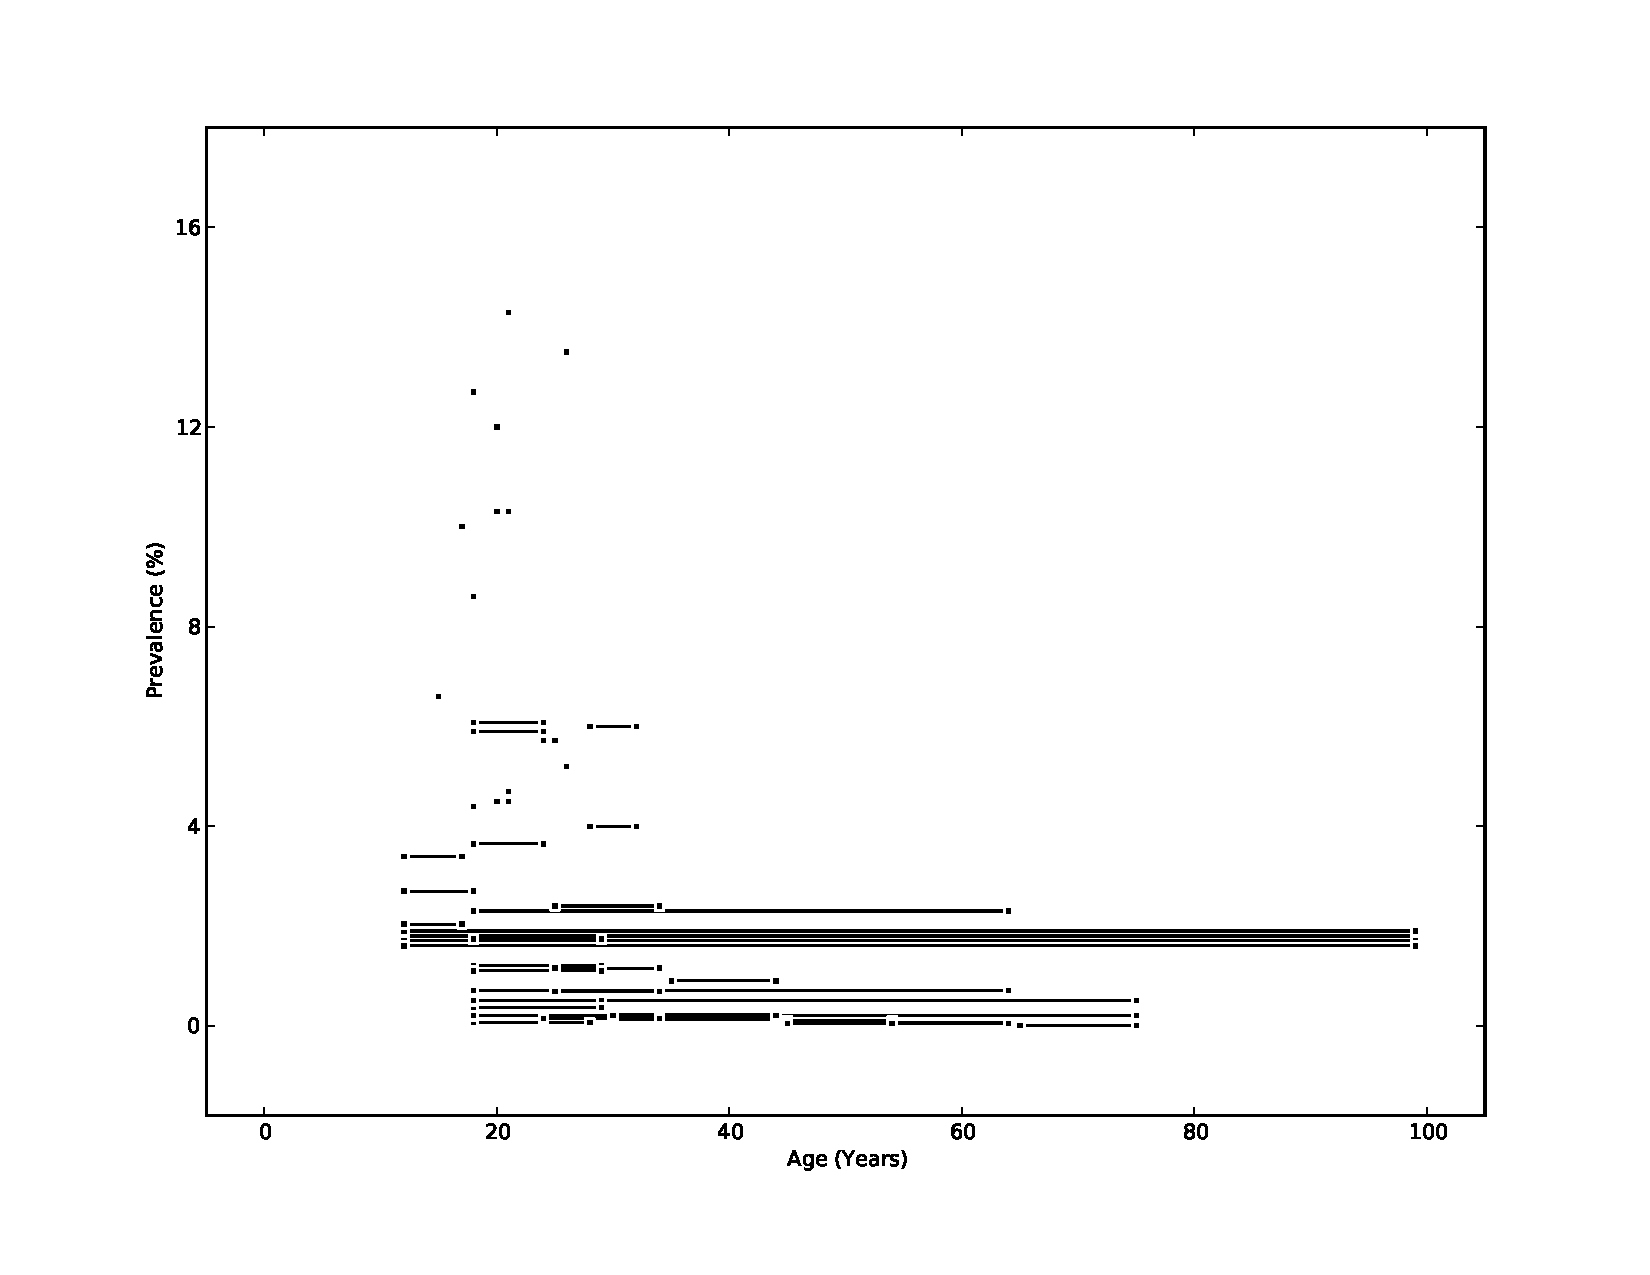
\includegraphics[width=\textwidth]{cannabis_dependence-data.pdf}
            \caption{Global prevalence data for cannabis dependence.}
            \label{fig:app-cannabis_data}
        \end{center}
    \end{figure}

As discussed in Chapter \ref{theory-age_pattern_model}, we model
age-specific hazards with spline models.  To be more specific, in this
case, the spline model takes the form of a continuous, piecewise
linear function, with ``knots'' where the function is non-linear
selected as part of the model.  These knots partition the age range
into intervals, and the choice of knots can be influential on the
resulting estimates.  In a setting where data is \emph{not} sparse and
noisy, estimates will not be very sensitive to choice of knots.
However, when working with sparse and noisy data, the number and
location of knots are important decisions as they can influence the
model results substantially.  Thus, the number of knots and locations
should be chosen a priori using expert knowledge concerning the
disease being modeled when the data are sparse and noisy.  It is also
important to consider additional knots and alternative configurations
of knots as a sensitivity analysis.

To demonstrate the importance of the number of knots in a spline
model, three models with differing numbers of knots are compared in
Figure \ref{fig:app-cannabis_knots}.  The original model for cannabis
dependence has knots at 0, 13, 17, 22, 30, 35, 40, 45, 50, 60, and
100.  The `less knot' model limits knots to ages 0, 13, 25, 65, and
100.  During the critical period of 13-50 years, the `more knot' model
has knots every three years \{13, 16, 19, \ldots, 43, 46, 49\} with
additional knots at \{0, 55, 60, 80, 100\}.  As seen in Figure
\ref{fig:app-cannabis_knots}, choosing too few or too many knots can
influence the model substantially.

    \begin{figure}[h]
        \begin{center}
            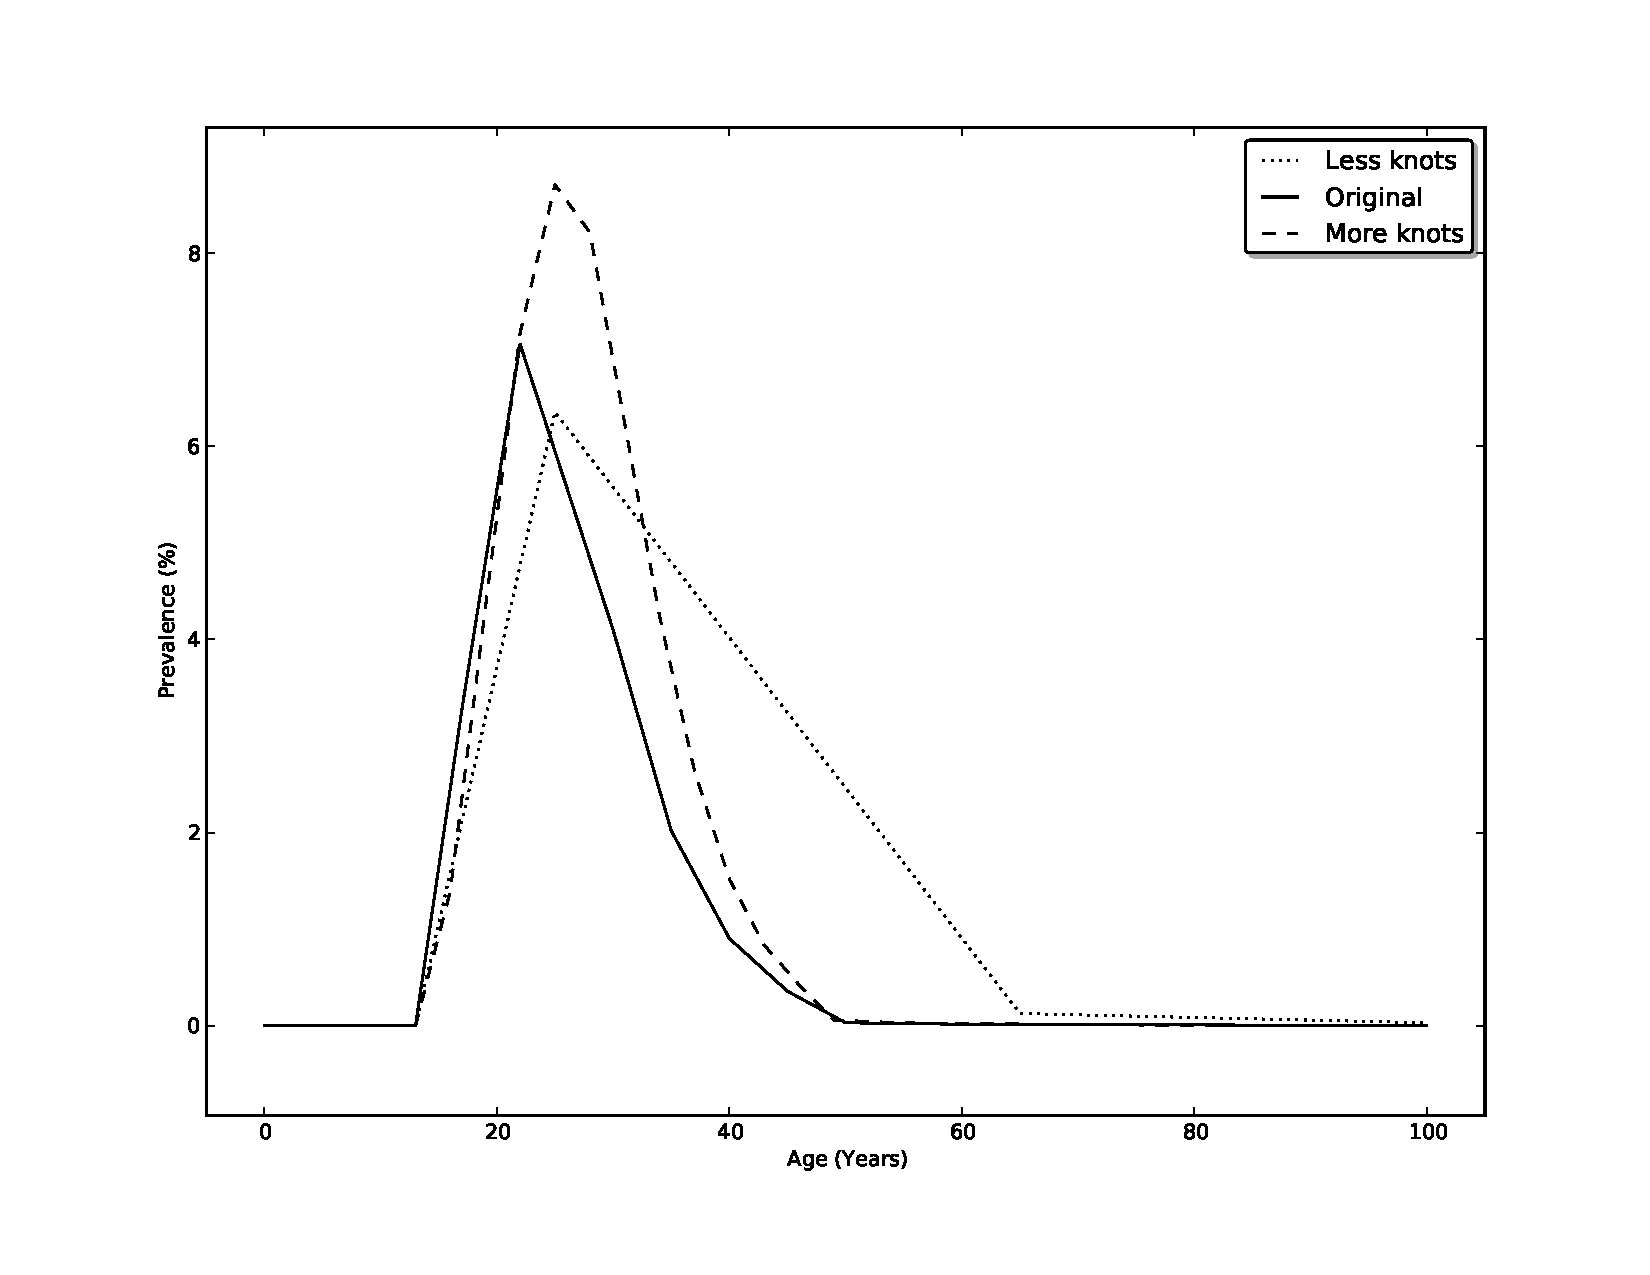
\includegraphics[width=\textwidth]{applications/cannabis_dependence-knots.pdf}
            \caption{Prevalence estimates of cannabis dependence using
              a single rate type model in the original model and
              models with less and more knots. }
        \label{fig:app-cannabis_knots}
        \end{center}
    \end{figure}

A penalized spline model with a smoothing parameter is another
solution to knot selection.  The model includes more knots but adds a
penalty to discourage the model from using more knots than necessary
for the data.  The smoothing parameter controls the roughness of the
estimating function and the fidelity of the estimates to the data,
making knot selection less influential as shown in Figure
\ref{fig:app-cannabis_smoothing}.  However, too much smoothing leads
to overcompression of the prevalence estimates, and results in
estimates that are not representative of the data.

    \begin{figure}[h]
        \begin{center}
            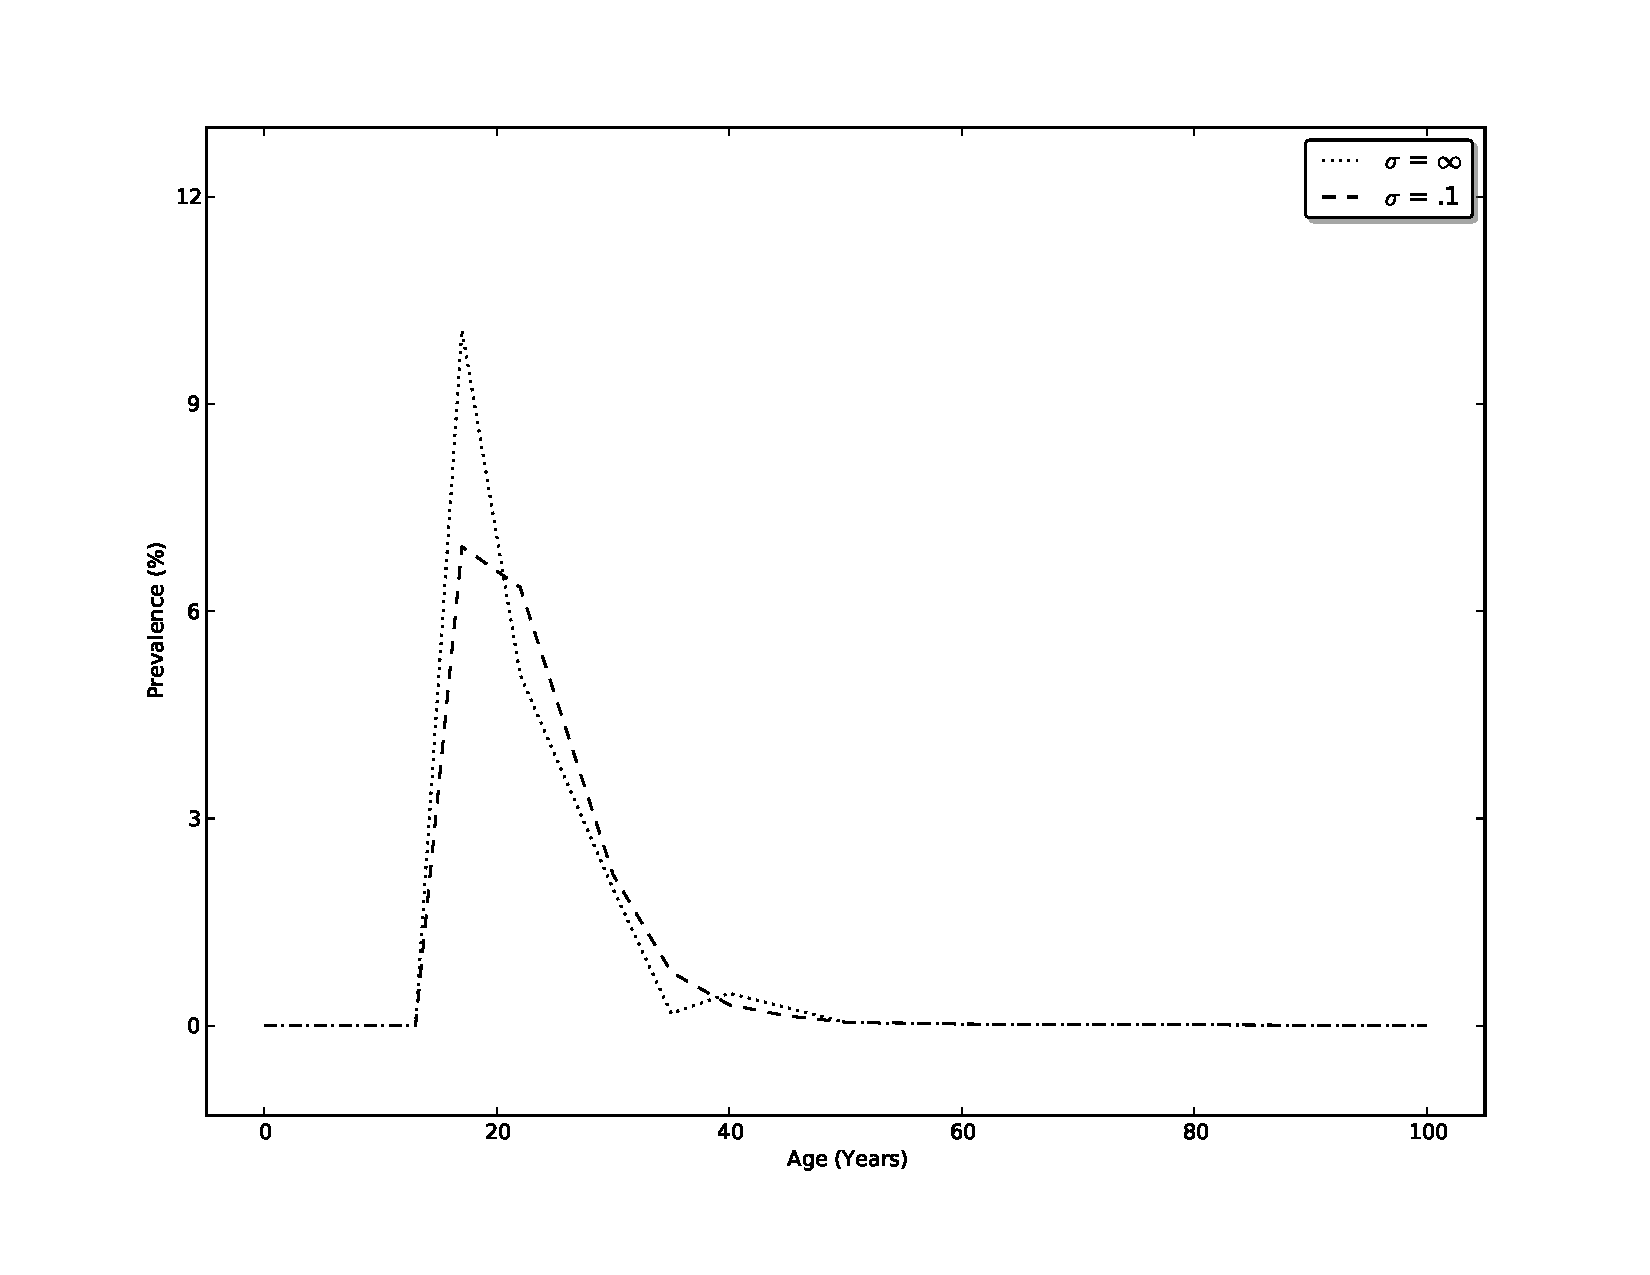
\includegraphics[width=\textwidth]{applications/cannabis_dependence-smoothing.pdf}
            \caption{Prevalence estimates from the original model
              using a penalized spline model with a smoothing
              parameter $\sigma$. }
        \label{fig:app-cannabis_smoothing}
        \end{center}
    \end{figure}

TK concluding paragraph, that summarizes the contents of this chapter
and reiterates the point: knot selection can be an influential part of
the model, and sensitivity analysis is necessary to determine if that
is the case.
